\documentclass[
    eng,
    % archivemode, % WERSJA ARCHIWALNA
]{lib/mgr}

% JĘZYK I FONTY
\usepackage{polski} 
\usepackage[utf8]{inputenc}
\usepackage[T1]{fontenc}

% GRAFIKA
\usepackage{graphicx}

% MATEMATYKA
\usepackage{mathtools}
\usepackage{amsfonts}

% TABELE
\usepackage{tabularx}
\usepackage{booktabs}
\usepackage{threeparttable}

% LISTY
\usepackage{enumitem}

% HIPERŁĄCZA
\usepackage{hyperref}
\usepackage{url}

% ZAŁĄCZANIE PLIKÓW
\usepackage{import}

% TIKZ
\usepackage{forest}

% DODATKI
\usepackage[toc,page,header,titletoc]{appendix}
    \renewcommand{\appendixtocname}{Dodatki}
    \renewcommand\appendixpagename{Dodatki}
    \usepackage{url}
\def\UrlBreaks{\do\/\do-}
\usepackage{rotating}
\usepackage{tabularx} % in the preamble
% \usepackage{bibentry}
% \usepackage{indentfirst}
\usepackage{listings}
\usepackage{pdflscape}
\usepackage{rotating, graphicx}
% DEBUG (odkomentować do debugu)
% \usepackage{showlabels}
\definecolor{folderbg}{RGB}{124,166,198}
\definecolor{folderborder}{RGB}{110,144,169}

\definecolor{filebg}{RGB}{200,100,100}
\definecolor{fileborder}{RGB}{100,50,50}

\def\Size{4pt}
\tikzset{
  folder/.pic={
    \filldraw[draw=folderborder,top color=folderbg!50,bottom color=folderbg]
      (-1.05*\Size,0.2\Size+5pt) rectangle ++(.75*\Size,-0.2\Size-5pt);  
    \filldraw[draw=folderborder,top color=folderbg!50,bottom color=folderbg]
      (-1.15*\Size,-\Size) rectangle (1.15*\Size,\Size);
  },
  file/.pic={
    \filldraw[draw=fileborder,top color=filebg!50,bottom color=filebg]
      (-\Size,-\Size) -| (\Size,.8*\Size) -- (0.4*\Size,1.4*\Size) -- (-\Size,1.4*\Size) -- cycle;
    \draw[fileborder]
      (\Size,.8*\Size) -| (0.4*\Size,1.4*\Size);
  },
}

\forestset{
    default preamble={
        for tree={
            font=\ttfamily,
            grow'=0,
            child anchor=west,
            parent anchor=south,
            anchor=west,
            calign=first,
            inner xsep=7pt,
            folder edges/.style={
                edge path={
                    \noexpand\path [draw, \forestoption{edge}]
                    (!u.south west) +(7.5pt,0) |- (.child anchor) pic {folder} \forestoption{edge label};
                }
            },
            file edges/.style={
                edge path={
                    \noexpand\path [draw, \forestoption{edge}]
                    (!u.south west) +(7.5pt,0) |- (.child anchor) pic {file} \forestoption{edge label};
                }
            },
            root file edges/.style={
                edge path={
                    \noexpand\path [draw, \forestoption{edge}] pic {folder}
                    (!u.south west) +(7.5pt,0) |- (.child anchor) pic {folder} \forestoption{edge label};
                }
            },
            folder edges,
            before typesetting nodes={
                if n=1 {
                    insert before={[,phantom]}
                }{}
            },
            fit=band,
            before computing xy={l=15pt},
        }  
    }
}
\input{src/hyphenation.tex}

\title{Uniwersalny system do wykrywania anomalii w danych wybranego typu}
\engtitle{System for general task of anomaly detection in data of a choosen type}
\author{Daniel Jabłoński}
\supervisor{dr Marek Bazan \newline Katedra Informatyki Technicznej}
%\guardian{mgr inż. Konrad Kluwak}
%\date{}

\field{% KIERUNEK, WYBIERZ JEDEN LUB DOPISZ WŁASNY
     Automatyka i Robotyka (AIR)
    % Elektronika (EKA)
    % Elektronika i telekomunikacja (EIT)
}
\specialisation{% SPECJALNOŚĆ, WYBIERZ JEDNĄ LUB DOPISZ WŁASNĄ
    % AIR
    % Robotyka (ARR)%
    % Komputerowe sieci sterowania (ARK)%
    % Systemy informatyczne w automatyce (ASI)%
    % Komputerowe systemy zarządzania\\procesami produkcyjnymi (ARS)%
    % EIT
    % Akustyka (ETA)%
    % Aparatura elektroniczna (EAE)%
    % Elektroniczne i komputerowe\\systemy automatyki (ESA)%
    % Zastosowania inżynierii komputerowej\\w technice (EZI)%
    Technologie informacyjne w systemach\\automatyki (ART)
}


\begin{document}
    % \bibliographystyle{plabbrv} 
    \bibliographystyle{siam}
    
    \maketitle
    % \import{src/}{dedication.tex}
    \tableofcontents 
    
    % \chapter{Wstęp}
\label{chap:wstep}
\section{Wprowadzenie}
\label{sec:wprowadzenie}

Yuval Noah Harari w swojej książce \textit{,,21 lekcji dla XXI wieku''} zwiastuje potencjał \textit{Big data}\footnote{Gromadzenie i przetwarzanie dużych zbiorów danych w celu uzyskania wartościowych informacji} w XXI wieku jako dobra, której wartość swoim potencjałem przyćmi tradycyjne dobra takie jak posiadanie ziemi, fabryk czy machin.
,,Harvard Business Review'' określa pozycję \textit{Data Scientist}\footnote{Specjalista analizujący dane w celu uzyskania pożądanych i wartościowych informacji} jako najbardziej pożądanej w XXI wieku \cite{davenport2012data}. Znaczenie eksploracji danych zwiększa się każdego dnia.
Ważną dziedziną tego procesu jest zadanie wykrywania anomalii. Początki badań nad metodą wykrywania anomalii w danych można znaleźć już w XIX w. \cite{edgeworth1887xli}. 
Wraz z rozwojem techniki komputerowej oraz zwiększoną ilością dostępnych danych, skuteczne metody wykrywania anomalii stały się pożądane. 
Detekcja anomalii w danych przekłada się na uzyskaniu cennych informacji w wielu dziedzinach takich jak:
\begin{itemize}
    \item W diagnostyce medycznej anomalny obraz z rezonansu magnetycznego może wskazać obecność nowotworu \cite{spence2001detection}
    \item W detekcji oszust finansowych takich jak kradzież karty kredytowej \cite{bolton2001unsupervised}
    \item W przemyśle do detekcji awarii sensorów \cite{dereszynski2011spatiotemporal} 
    \item W zabezpieczeniach sieciowych do wykrywania włamań do sieci \cite{garcia2009anomaly}
\end{itemize} 

Wykrywanie anomalii odnosi się do problemu znajdowania obserwacji, które odbiegają zachowaniem od normy. Słownik języka polskiego definiuje anomalię jako: ,,odchylenie od normy'' \cite{pwn}. 
W literaturze można spotkać się z określeniami takich punktów jako: nieprawidłowość, obserwacja odstająca, niezgodność, dewiacja. \cite{aggarwal2017outlier}. Z czego najczęstszym określeniem w danym kontekście jest anomalia oraz obserwacja odstająca, które czasami używane są zamiennie. Związane jest to z podejściem zakładającym, że problem wykrywania anomalii jest uczeniem nienadzorowanym. Do detekcji anomalii bazujemy na metodach statystycznych w celu znalezieniu elementów odstających z założeniem, że owe punkty będą anomaliami. Jest to dominujące założenie w literaturze \cite{emmott2015meta}. Drugim podejściem jest modelowanie osobno normalnych i anomalnych punktów. Jednakże, to podejście wymaga znajomości procesu powstania obu typów punktów w zbiorze danych lub wystarczającą liczbę oznaczonych danych szkoleniowych. Co w problemach wymagających detekcji anomalii, gdzie operujemy na nieoznaczonych danych oraz nie znamy procesu generującego anomalne punkty, jest podejściem nieprzydatnym. W związku z tym w niniejszej pracy do detekcji punktów anomalnych wykorzystamy podejście bazujące na detekcji elementów odstających.
% Wykrywanie anomalii odnosi się do problemu znajdywania punktów, które odbiegają zachowaniem od spodziewanego wzoru. Takie punkty nazywane są anomaliami, obserwacjami odstającymi, wyjątkami, niespodziankami. W literaturze najczęściej wykorzystuje się zwroty anomalia oraz obserwacja odstająca. Zwroty te często używane są zamiennie. 
\section{Cel pracy}
Celem pracy jest opracowanie oraz implementacja uniwersalnego systemu internetowego służącego do detekcji anomalii dla dowolnych zbiorów danych obserwacji statystycznych (bez etykiet). System ma pozwalać na przesłanie danych w popularnych formatach CSV oraz JSON. Przetworzeniu uzyskanych danych m.in. oczyszczeniu danych z brakujących wartości oraz normalizacji danych. Stworzeniu raportu z działania systemu oraz zapewnieniu użytkownikowi oczyszczonych danych z anomalii w formacie, w którym te dane zostały przesłane. System powinien być jak najprostszy w obsłudze, szybki w działaniu oraz zapewniać kluczowe informacje pozwalającemu użytkownikowi na dalszą analizę uzyskanych wyników. 
System ma zapewnić użytkownikowi nieposiadającemu wiedzy na temat wykrywania anomalii automatyzację procesu wyboru algorytmu detekcji oraz jego parametrów w celu zwiększenia skuteczności detekcji.


Praca składa się pięciu rozdziałów. Rozdział pierwszy ma za zadanie wprowadzić czytelnika w tematykę zagadnienia. Rozdział drugi dogłębnie przedstawić aktualne metody na detekcje anomalii. Rozdział trzeci poświęcony jest omówieniu stworzonego systemu. Rozdział czwarty jest dogłębną analizą poprawności działania systemu. Ostatni rozdział podsumowuje całość pracy oraz prezentuje możliwości rozwoju systemu. 

    % \chapter{Wykrywanie anomalii}
\label{chap:OD}

\begingroup
\leftskip4em
\rightskip\leftskip
\noindent
\textbf{Abstrakt} W poprzednim rozdziale przyjęto podejścia wykrywania anomalii za pomocą detekcji obserwacji odstających. W tym rozdziale przybliżono teorię oraz dokonano przeglądu i porównania algorytmów wykorzystywanych do detekcji obserwacji odstających. Jak również przedstawiono opis proponowanego rozwiązania wykorzystanego w celu doboru algorytmu oraz jego parametrów, którego zadaniem jest zapewnienie optymalnej metody detekcji anomalii dla zbioru danych.
\par
\endgroup

\section{Definicja anomalii (obserwacji odstającej)}
Obserwacje odstające to punkty, które nie odpowiadają wzorcowi w zbiorze danych. Barnett i Lewis definiują obserwację odstającą następująco: ,,Obserwacja odstająca jest to obserwacja, której obecność jest różna od pozostałych obserwacji'' \cite{barnett1984outliers}. Rysunek \ref{fig:anomalia} obrazuje przykład obserwacji odstających (anomalii) dla dwuwymiarowego zbioru danych. Zbiór danych posiada przestrzeń {$N_1$}, większość punktów znajduje się wewnątrz tej przestrzeni. Punkty wystarczająco oddalone od przestrzeni $N_1$: $o_1$, $o_2$, $o_3$ -- sklasyfikowane są jako obserwacje odstające (anomalie).
\begin{figure}[h]
    \centering
    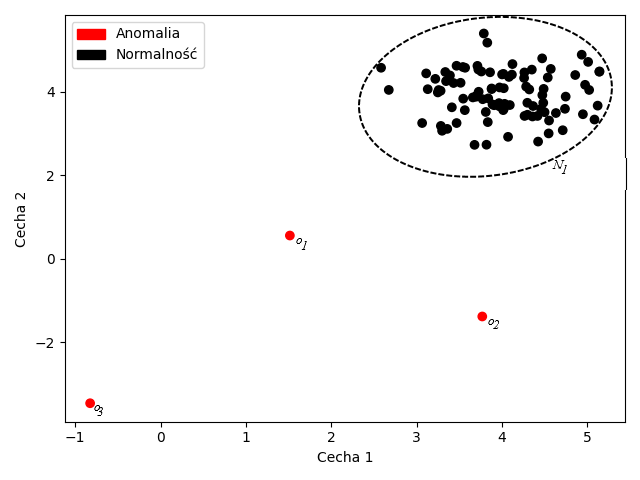
\includegraphics[width=.7\textwidth]{chapters/istniejace/images/anomalia.png}
    \caption{Prosty przykład anomalii w dwuwymiarowym zbiorze danych.}
    \footnotesize{źródło: Opracowanie własne}
    \label{fig:anomalia}
\end{figure}

\section{Zadanie detekcji anomalii}
W pracy rozważamy nienadzorowane zadanie detekcji anomalii na zbiorze $N$ punktów $x_1,...,x_N$ każdy punkt jest d-wymiarowym wektorem liczb rzeczywistych. Zbiór danych składa się z obserwacji poprawnych i anomalnych, jednakże zbiór nie posiada wektora $y_1,..,y_N$ -- klasyfikującego obserwację do obserwacji poprawnych lub anomalnych. Celem zadania detekcji anomalii jest wykrycie punktów anomalnych w danym zbiorze.

\section{Różnice w podejściu detekcji anomalii}

\subsection{Wykrywanie anomalii lokalnych a globalnych}
\label{sub:loc_glob}
Podejście dotyczy wyboru zakresu zbioru jako zbioru odniesienia dla rozpatrywania odstawania danej obserwacji. Główne podejścia to podejście globalne oraz lokalne. Rysunek \ref{fig:anomalie_glob_lok} obrazuje prosty dwuwymiarowy zbiór danych z dwoma klastrami (skupieniami) poprawnych obserwacji: $c_1$ i $c_2$. Dla punktów $x_1 $ oraz $x_2$ klasyfikacja jako anomalie jest możliwa wizualnie. Oba punkty są znacząco oddalone od gęstych obszarów obserwacji. Są to anomalie globalne. Rozpatrując wszystkie obserwacje zbioru punkt $x_3$ mógłby być uznany za poprawną obserwację należącą do klastra $c_2$, jednak kiedy rozpatrzymy podzbiór punktów w sąsiedztwie klastra $c_2$ (zbiór odniesienia), punkt $x_3$ może być uznany za anomalię. Jest to przykład anomalii lokalnej. Zatem anomalia lokalna jest to obserwacja, której odchylenie od normy (anomalność) rozpatrywane jest w obszarze najbliższego sąsiedztwa (zbioru odniesienia). 
\begin{itemize}
    \item Podejście globalne 
    \begin{itemize}
        \item Zbiór odniesienia obejmuje wszystkie obserwacje
        \item Założenie o istnieniu jeden prawidłowego mechanizmu generującego normalne punkty.
        \item Problem: występowanie anomalii lokalnych lub więcej niż jeden prawidłowy mechanizm generujący punkty mogą wypaczyć wynik detekcji
    \end{itemize}
    \item Podejście lokalne 
    \begin{itemize}
        \item Zbiór odniesienia jest podzbiorem całego zbioru
        \item Brak założenia o liczbie mechanizmów generujących.
        \item Problem: wybór odpowiedniego podzbioru jako zbioru odniesienia
    \end{itemize}
\end{itemize}

\begin{figure}[h]
    \centering
    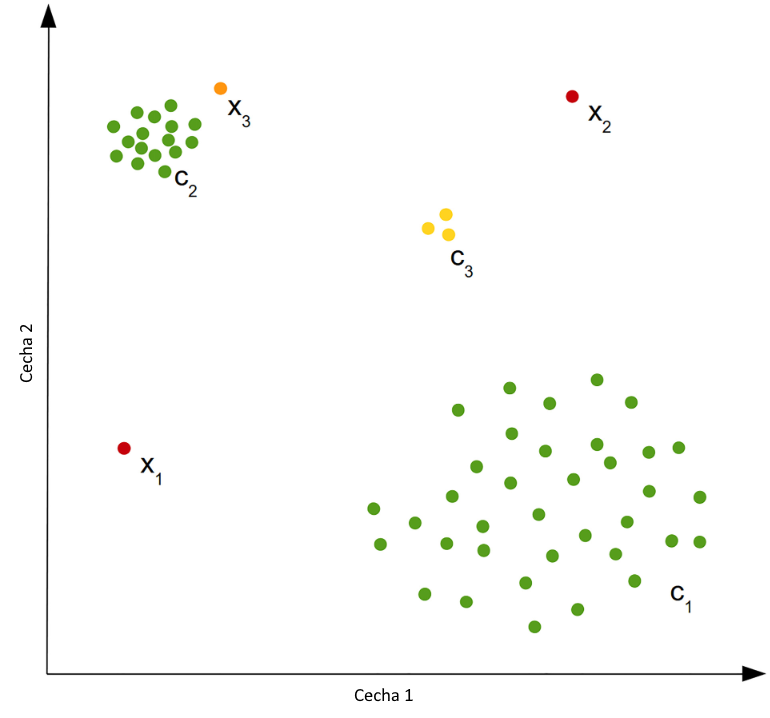
\includegraphics[width=.65\textwidth]{chapters/istniejace/images/mikro_cluste.png}
    \caption{Przykład anomalii globalnych ($x_1, x_2$), lokalnej $x_3$ oraz mikro klastra $c_3$. }
    \footnotesize{źródło: Opracowanie własne na podstawie \cite{goldstein2016comparative}}
    \label{fig:anomalie_glob_lok}
\end{figure}

\subsection{Wynik metody}
\label{sec:score}
Ważnym aspektem dla zadania wykrywania anomalii jest sposób oceny każdej obserwacji. Dane wyjściowe metody mogą przypisywać obserwacji wynik anomalności na dwa warianty:
\begin{itemize}
    \item binarny: przypisanie obserwacji etykiety. Klasyfikacja obserwacji jako anomalii lub poprawnej obserwacji w zbiorze
    \item ciągły: dla każdej obserwacji obliczana jest wartość anomalności np. prawdopodobieństwo obserwacji jako anomalii
\end{itemize}
Podejście przypisujące wynik anomalności w sposób ciągły (wartość anomalności) jest podejściem wszechstronnym. Wykorzystując podejście osoba analizująca dane może za pomocą np. progu wartości anomalności, otrzymać binarną etykietę obserwacji, dostosowując próg dla danej dziedziny.
Wiele podejść opartych na przypisywaniu wyniku anomalności skupia się na wyznaczeniu grupy n-obserwacji o najwyższym wyniku (parametr n często podawany jest przez użytkownika np. procent kontaminacji zbioru danych). 
Podejście oparte na ciągłym wyniku anomalności punktu przydatne jest w rozważaniu mikro klastrów, czyli małych regularnych klastrów. Rysunek \ref{fig:anomalie_glob_lok} obrazuje mikro klaster $c_3$. Algorytm detekcji anomalii powinien przypisać punktom klastra wartość anomalności wyższą od normalnych obserwacji oraz mniejszą od anomalii globalnych. Przykład pokazuje, że podejście przypisywania ciągłej wartości anomalności punktu jest podejściem bardziej użytecznym od binarnej klasyfikacji zwłaszcza w dalszej analizie danych. 

\subsection{Rodzaje anomalii}
% Punktowe, collective i contextual - można wszystko z punktowych które są dominujące w unsupervised detection
W detekcji anomalii wyróżnia się trzy rodzaje anomalii: anomalie punktowe, anomalie zgrupowane oraz anomalie kontekstowe.
Większość dostępnych algorytmów detekcji anomalii dla uczenia nienadzorowanego opiera się na wykrywaniu anomalii punktowych. Detekcja anomalii zgrupowanych została przedstawiona na rysunku \ref{fig:anomalie_glob_lok} i opisana w sekcji \ref{sec:score} -- mikro klaster $c_3$.
Anomalie kontekstowe są to anomalie najczęściej spotykane w szeregach czasowych. Dotyczy to punktów, które mogą być uznane za poprawne obserwacje, jednak rozpatrywane w kontekście charakteru zbioru danych zostaną uznane za anomalie. Weźmy przykład pomiaru temperatury w skali roku we Wrocławiu. Temperatura 25$^{\circ}$C wydaje się poprawnym odczytem temperatury, jednak w kontekście miesiąca np. stycznia. Tak wysoka temperatura jest anomalią.

Szczęśliwie można wykorzystać algorytmy detekcji anomalii punktowych do wykrywania anomalii zgrupowanych i kontekstowych. 
Detekcja różnych typów anomalii wymaga obróbki danych m.in. przekształcenia zbioru danych reprezentującego cechy z wykorzystaniem korelacji, agregacji oraz grupowania \cite{goldstein2014behavior} w celu analizy obserwacji jako anomalii punktowych.

W pracy skupiono się na problemach detekcji anomalii punktowych, wykorzystując bazę zbiorów danych ODDS \cite{ODDS}. Baza zawiera zbiory danych już przygotowanych do zadania detekcji anomalii punktowych.



% \section{Proponowane rozwiązanie: MetaOD}
% 
\section{Wykorzystywane algorytmy}
\subsection{ABOD}
\subsection{HBOS}
\subsection{LOF}
\subsection{COF}
\subsection{Isolation Forest}
\subsection{kNN}
\subsection{LODA}
\subsection{OCSVM}

    % \chapter{Proponowana metoda detekcji anomalii}
\begingroup
\leftskip4em
\rightskip\leftskip
\noindent
\textbf{Abstrakt} W rozdziale przedstawiono proponowane rozwiązanie doboru modelu detekcji anomalii pozwalające na automatyzację tego procesu. Rozdział zawiera również opis algorytmów wraz z parametrami, składających się na przestrzeń bazową modeli.
\par
\endgroup
\section{Proponowane rozwiązanie: MetaOD}
\section{Wykorzystywane algorytmy}
W sekcji zostanie przybliżone działanie algorytmów(Rysunek \ref{fig:typy}) z uwzględnieniem znaczenia parametrów dobranych przez MetaOD.
Wszystkie algorytmy implementowane są z wykorzystaniem biblioteki \textit{Python Outlier Detection} (PyOD) \cite{zhao2019pyod}
\begin{figure}
    \centering
    \includegraphics[width=\textwidth]{chapters/istniejace/images/TypyAlgorytmów(1).png}
    \caption{Wykorzystywane algorytmy z podziałem na metodologię}
    \label{fig:typy}
\end{figure}

\subsection{OCSVM}
\textit{One-Class SVM} [Jednoklasowa maszyna wektorów nośnych] (OCSVM) \cite{ocsvm}. OCSVM jest binarną metodą klasyfikacji odwzorowującą dane wejściowe z wykorzystaniem funkcji jądrowej na przestrzeń wielowymiarową w poszukiwaniu hiperpłaszczyzny separującej poprawne obserwacje od anomalii.  
% Model jądrowy:
% \begin{equation}
%     f(x) = \sum_{i=1}^{N} \alpha _i y_iK(x_i,x)+b
% \end{equation}
% gdzie $K$ jest funkcją jądrową:
Funkcje jądrowe:
\begin{align*}
    Liniowa: x^Tx_i \\
    Wielomianowa: (\gamma x^Tx_i+c)^n \\
    RBF: exp(-\gamma ||x-x_i||^2) \\
    Sigmoidalna: tgh(\gammax^Tx_i+c)
\end{align*}
\label{eq:funjadro}

\subsection{kNN}
\textit{k-Nearest Neighbors}[Algorytym k najbliższych sąsiadów] (kNN) \cite{knn} opiera się na wnioskowaniu, że poprawne obserwacje będą w sąsiedztwie innych poprawnych obserwacji. Natomiast anomalie będą znacząco oddalone od klastrów normalnych obserwacji. Dla każdego elementu obliczamy metrykę do k = 1,...,N sąsiada. Wynik anomalności elementu zależy od metody (wybrana przez MetaOD):
\begin{itemize}
    \item \textit{largest} - anomalność punktu jest odległością do k-sąsiada (najdalej oddalonego)
    \item \textit{mean} - anomalność punktu jest średnią ze wszystkich odległości do sąsiadów
    \item \textit{median} - anomalność punktu jest medianą wszystkich odległości do sąsiadów
\end{itemize}

\subsection{LOF}
\textit{Local Outlier Factor}(LOF) \cite{lof} algorytm w odróżnieniu od algorytmu kNN rozpatruje lokalną gęstość względem sąsiadów. Podejście odnosi się do wad metod opartych na metryce (anomalie globalne) w przypadkach zbiorów danych o różnych gęstościach klastrów poprawnych obserwacji(Rysunek \ref{fig:anomalie_glob_lok}).
W celu obliczenia anomalności punktu należy dokonać 3 kroków:
\begin{enumerate}
    \item Dla rozpatrywanego punktu x, należy znaleźć k najbliższych sąsiadów
    \item Rozpatrując k najbliższych sąsiadów $N_k$, wyznaczyć zagęszczenie w k-sąsiedztwie punktu x obliczając \textit{local reachability density}(LRD): 
    \begin{equation}
        LRD_k(x) = 1/\Bigg(\frac{ \sum\limits_{o \in N_k(x)} d_k(x,o) }{|N_k(x)|}\Bigg)
    \end{equation}
    gdzie $d_k(\cdot)$ oznacza \textit{reachability distance}
    \item Ostatecznie obliczamy wartość LOF porównując LRD punktu $x$ z LRD k-sąsiada:
    \begin{equation}
        LOF(x) = \frac{ \sum\limits_{o \in N_k(x)} \frac{LRD_k(o)}{LRD_k(x)} }{|N_k(x)|}
    \end{equation}
\end{enumerate}
Wynik LOF jest stosunkiem
% współczynnikiem lokalnej gęstości.
Jeżeli wartość $LOF(x)>1$ oznacza to małą lokalną gęstość(anomalia lokalna). 
$LOF(x) \approx 1$ oznacza, że lokalna gęstość punktu x jest zbliżona do sąsiadów.

\subsection{COF}
\textit{Connectivity based Outlier Factor}(COF) \cite{cof} algorytm COF jest zbliżony do LOF, główną różnicą wybór k najbliższych sąsiadów (Rysunek \ref{fig:lcof}. LOF wybiera k najbliższych sąsiadów korzystając z odległości Euklidesowej, tworząc wokół analizowanego punktu sferę. COF tworzy zbiór k-sąsiadów dla punktu x wybierając najpierw najbliższego sąsiada dodając go do zbioru. Następnie wybiera punkt najbliższy do dowolnego elementu istniejącego zbioru k-sąsiadów do momentu aż zbiór będzie miał k elementów. Tworząc swojego rodzaju łańcuch k-sąsiadów. Obliczanie lokalnej gęstości przebiega w ten sam sposób co w LOF -- stosunek \textit{chaining distance} dla punktu x do średniej z \textit{chaining distance} dla k-sąsiadów :
\begin{equation}
    COF_k(x) = \frac{|N_k(x)| \cdot ac-dist_{N_K(x)}(x)}{\sum\limits_{o \in N_k(x)}ac-dist_{N_k(o))}(o)}
\end{equation}
gdzie $ac-dist_{N_k(x)}$ jest średnią odległością punktu x 
\begin{figure}
    \centering
    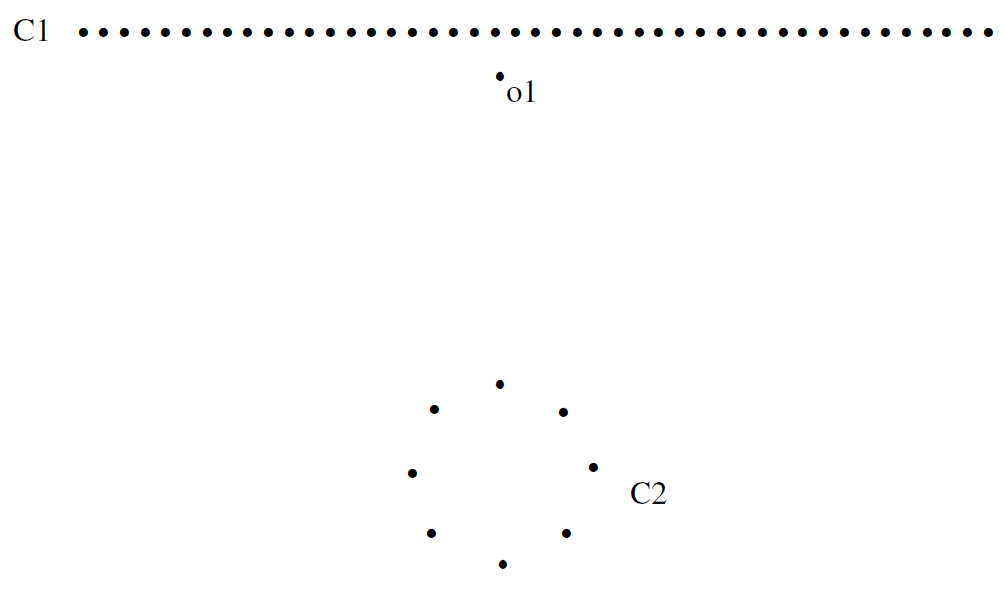
\includegraphics[width=.6\textwidth]{chapters/MetaOD/images/cof.png}
    \caption{Zbiór dla którego detekcja anomalii algorytmem LOF nie powiedzie się \cite{cof}}
    \label{fig:cof}
\end{figure}

\begin{figure}
    \centering
    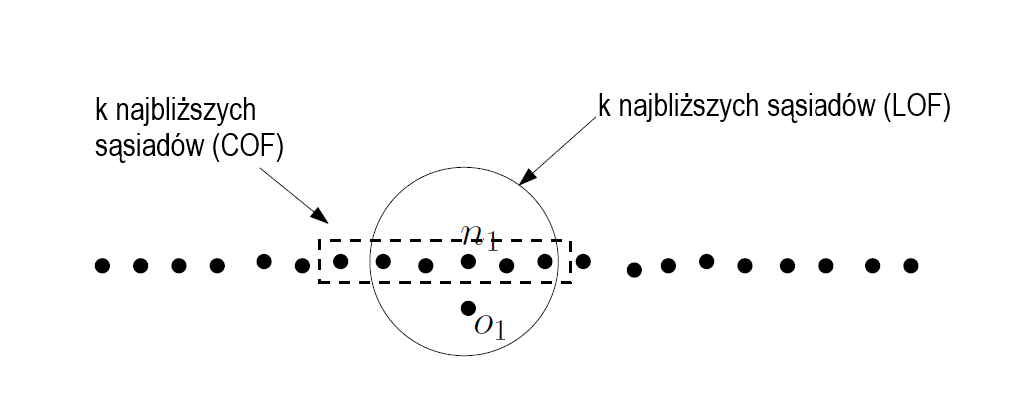
\includegraphics[width=.6\textwidth]{chapters/MetaOD/images/lvcof.png}
    \caption{Różnica w wyborze k najbliższych sąsiadów dla COF i LOF (k=5) \cite{chandola2009anomaly}}
    \label{fig:lcof}
\end{figure}

\subsection{ABOD}
\textit{Angel-based Outlier Detection}(ABOD) \cite{abod} W wielowymiarowych przestrzeniach kąty są stabilniejsze niż metryka, spowodowane jest to "przekleństwem wymiarowości". Rezultatem badań na temat zagadnienia "przekleństwa wymiarowości"\cite{curse} jest wniosek, że najdalszy punkt i najbliższy punkt zbiegają do 0 ze wzrostem wymiarów:
\begin{equation}
\lim_{d\to\infty} \frac{dist_{max} - dist_{min}}{dist_{min}} \longrightarrow 0
\end{equation}
Z tego powodu np. w grupowaniu dokumentów tekstowych jako miary podobieństwa wykorzystuje się miarę kosinusową \cite{huang2008similarity}. Algorytm ABOD zamiast metryki między punktami w sąsiedztwie porównuje kierunek wektorów skierowanych wychodzących z rozpatrywanego punktu $x$. Standardowy ABOD rozpatruje wszystkie punkty w zbiorze w odniesieniu do analizowanego punktu, jest to podejście o wysokiej złożoności obliczeniowej $O(n^3)$. W celu zmniejszenia złożoności obliczeniowej w pracy wykorzystamy FastABOD, który rozpatruje k-sąsiadów. Rysunek \ref{fig:abod} obrazuje założenie algorytmu ABOD, który do oceny anomalności punktu stosuje współczynnik \textit{Angle-based outlier factor}(ABOF):
\begin{equation}
    ABOF(x) = Var\frac{\langle \overrightarrow{xy}, \overrightarrow{xz} \rangle⟩}{\big\| \overrightarrow{xy\big\|}\big\| \overrightarrow{xz}\big\|},y,z \in B
\end{equation}
gdzie $B$ jest odpowiednio dobranym zbiorem, jako iż używamy FastABOD jest to zbiór k-sąsiadujących punktów. Czym niższy ABOF tym większe podejrzenie anomalii (PyOD w celu zachowania konwencji -- większa wartość wyjściowa algorytmu oznacza wyższą anomalność obserwacji -- stosuje przeciwność ABOF tzn. -ABOF)
\begin{figure}
    \centering
    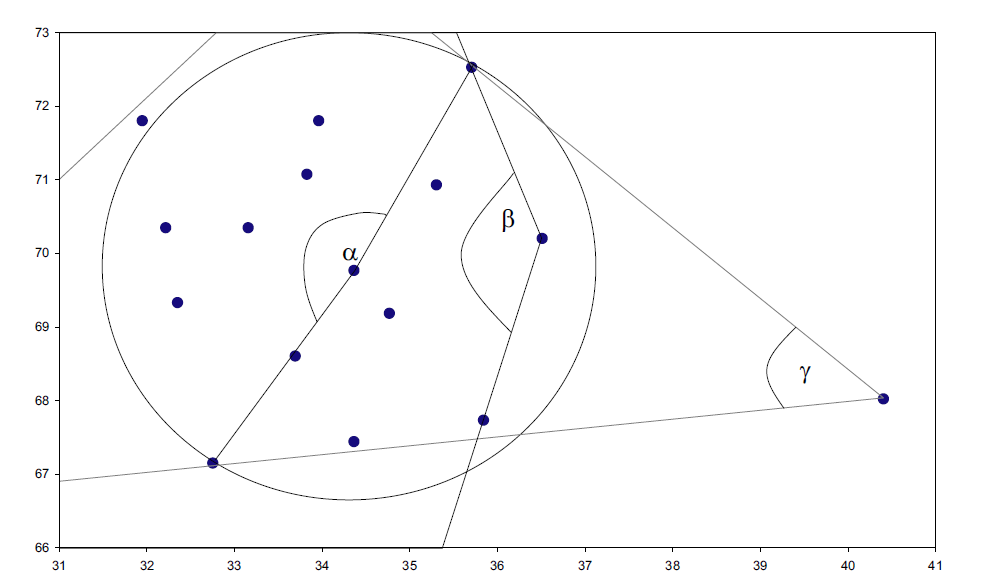
\includegraphics[width=.8\textwidth]{chapters/MetaOD/images/abod.png}
    \caption{Intuicja kierująca algorytmem ABOD \cite{abod}}
    \label{fig:abod}
\end{figure}

\subsection{HBOS}
\textit{Histogram-based Outlier Detection} (HBOS) \cite{hbos}

\subsection{LODA}
\textit{Lightweight Online Detector of Anomalies}(LODA) \cite{loda}

\subsection{IForest}
\textit{Isolation Forest}(IForest) \cite{iforest}
\label{sub:IF}

    % \chapter{System wykrywania anomalii}

\section{Wytyczne projektowe}
 Uniwersalny system wykrywania anomalii ma za zadanie ułatwić korzystającemu detekcję anomalii dla dowolnego zbioru danych statystycznych. W tym celu najważniejszą funkcją systemu jest automatyzacja wyboru optymalnego modelu detekcji anomalii. System po procesie analizy danych ma wizualizować wynik detekcji w sposób przejrzysty i zrozumiały dla korzystającego.    
\subsection{Wymagania funkcjonalne}
\begin{itemize}
    \item Przesłanie pliku zawierającego zbiór danych w formatach: JSON, CSV
    \item Oczyszczenie danych z brakujących wartości oraz wyskalowanie 
    \item Wybór optymalnego modelu (algorytm i parametry) 
    \item Detekcja anomalii w zbiorze danych z wykorzystaniem wybranego przez system modelu
    \item Utworzenie oczyszczonego zbioru danych z anomalii (wartość anomalności w 99. per centylu)
    \item Utworzenie zbioru danych z wartością anomalności dla każdej obserwacji
    \item Stworzenie raportu z przebiegu i wyniku detekcji anomalii
\end{itemize}
\subsection{Wymagania niefunkcjonalne}
\begin{itemize}
    \item Zbiory danych do pobrania (oczyszczone i zawierające wartość anomalności) powinny być w formacie przesłanych danych
    \item System powinien być jak najbardziej intuicyjny i prosty w obsłudze
    \item Raport powinien zawierać niezbędne informacje potrzebne do dalszej analizy przez użytkownika
    \item System oraz raport powinny być przystępne dla użytkownika bez wiedzy na temat detekcji anomalii
\end{itemize}

\section{Analiza technologiczna}
\subsection{Wykorzystane technologie oraz biblioteki}
System powstał z wykorzystaniem języka programistycznego Python 3.7. Jest to prosty do nauczenia, przejrzysty, a zarazem wszechstronny język programistyczny o rosnącej popularności zwłaszcza w środowisku uczenia maszynowego. Do stworzenia aplikacji webowej wykorzystano mikro-framework Flask 1.1.2. Do projektowania struktury i interfejsu graficznego strony internetowej wykorzystano: HTML, JavaScript oraz biblioteki CSS -- Bootstrap.
Do wyboru optymalnego modelu detekcji anomalii wykorzystano bibliotekę MetaOD, którą opisano w sekcji \ref{sec:MetaOD}. Do detekcji anomalii w zbiorze danych, wykorzystując algorytmy z przestrzeni bazowej modeli, skorzystano z gotowych implementacji algorytmów zawartych w bibliotece PyOD. 
Do analizy oraz przechowywania danych w strukturach danych użyto pakietu Pandas (tabela danych) oraz Numpy(tablice). Do skalowania zbioru danych wykorzystano bibliotekę Scikit-learn. Matplotlib został wykorzystany jako kreator wykresów pudełkowych oraz histogramów.

% Funkcjonalność aplikacji webowej została napisana w języku Python 3.7 z wykorzystaniem frameworku Flask 1.1.2.
% Interfejs graficzny powstała z użyciem języków HTML oraz JavaScript.
% Interfejs graficzny wykorzystuje bibliotekę CSS -- Bootstrap. 
% Do przechowywania danych w strukturach danych wykorzystano biblioteki: NumPy(tablice) oraz Pandas(tabela danych). 
% Detekcje anomalii przeprowadzona została z wykorzystaniem MetaOD i PyOD. 
% Do tworzenia wykresów wykorzystano bibloteki Matplotlib
% % \begin{itemize}
% %     \item Python 3.7 - 
% %     \item HTML
% %     \item Flask
% %     \item Bootstrap - bibloteka CSS, służąca do tworzenia interfejsu graficznego strony internetowej. 
% %     % \item Jinja2 
% %     \item PyOD
% %     \item MetaOD
% %     \item Sklearn
% %     \item FPDF
% %     \item Matplotlib
% %     \item Pandas
% %     \item Numpy
% % \end{itemize}
\subsection{Wykorzystane narzędzia programistyczne}
Zintegrowanym środowiskiem programistycznym wykorzystanym przy tworzeniu aplikacji był PyCharm Professional, czeskiej firmy JetBrains. To zaawansowane i wszechstronne środowisko ułatwia proces pisania kodu źródłowego, testowania oraz rozwijania oprogramowania. Posiada graficzny debugger ułatwiający identyfikację błędów. Wspiera pisanie aplikacji webowych. Posiada integrację z systemem kontroli wersji Git, wykorzystanego przy produkcji systemu do tworzenia kolejnych wersji rozwijanego projektu. Dzięki czemu implementacja nowych funkcjonalności odbywa się bez obawy utraty działającej wersji systemu.

% \section{Architektura systemu}
\section{Implementacja funkcjonalności}

\subsection{Uzyskanie danych}
System rozpoczyna działanie od strony startowej, na której klient może wybrać plik z danymi, które chce poddać zadaniu detekcji anomalii. Plik musi mieć rozszerzenie CSV lub JSON. Po naciśnięciu przycisku ,,Analizuj'' następuje przesłanie pliku do systemu. System sprawdza zgodność rozszerzenia pliku, jeżeli rozszerzenie jest obsługiwane, następuje zapisanie pliku na serwerze.
\begin{figure}
    \centering
    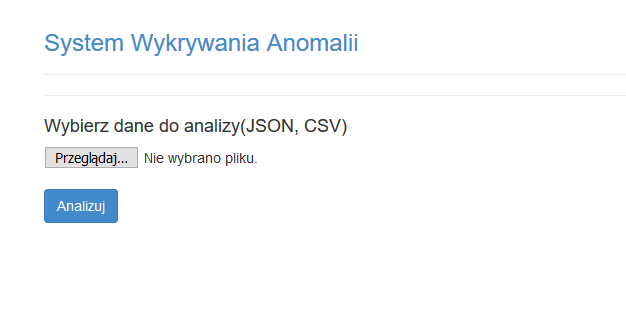
\includegraphics[width=\textwidth]{chapters/projekt/images/index.png}
    \caption{Strona startowa systemu wykrywania anomalii}
    \footnotesize{źródło: Opracowanie własne}
    \label{fig:my_label}
\end{figure}
\subsection{Przygotowanie danych}
Po zapisaniu pliku na serwerze następuje wczytanie danych z wykorzystaniem biblioteki Pandas. Wczytane dane są weryfikowane pod kątem brakujących wartości, jeśli zbiór danych zawiera brakujące wartość, system w miejsce brakującej wartości wstawia średnia z cechy (kolumny). System również dokonuje standaryzacji zbioru danych, wykorzystując funkcje biblioteki Scikit-learn -- \textit{MinMaxScaler}, która skaluje obserwację według wzoru:
\begin{equation}
       X_{std} = \frac{X - X_{min}}{X_{max} - X_{min}} 
\end{equation}
%     % X_{scaled} = X_{std} \cdot (max - min) + min
%  \end{gather}
 gdzie min, max są to minimalne i maksymalne wartości obserwacji. \textit{MinMaxScaler} został wybrany ze względu na największą skuteczność dla zestawu testowych zbiorów danych (podsekcja \ref{minimen}).
%  % \begin{sidewaystable}
%     \centering
\begin{table}[]
    \centering
\begin{tabularx}{\textwidth}{lXXXXX}
      Zbiór & Dane oryginalne & Robust Scaler & Standard Scaler & MinMax Scaler & Power Transformer \\ \hline
arrhythmia &               0.7480 &                  0.7527 &            0.7685 &      0.8093 &      0.7619 \\
    cardio &               0.5474 &                  0.6150 &            0.8604 &      0.9109 &      0.3830 \\
     glass &               0.6249 &                  0.4016 &            0.7122 &      0.7518 &      0.6076 \\
ionosphere &               0.8336 &                  0.8308 &            0.8065 &      0.8678 &      0.8481 \\
    letter &               0.8790 &                  0.8096 &            0.8976 &      0.8411 &      0.9062 \\
    lympho &               0.9977 &                  0.9930 &            0.9953 &      0.9941 &      1.0000 \\
      musk &               0.9460 &                  0.9994 &            0.7267 &      0.9923 &      0.1024 \\
 optdigits &               0.7431 &                  0.4615 &            0.5380 &      0.4757 &      0.4856 \\
 pendigits &               0.6975 &                  0.7786 &            0.6792 &      0.7218 &      0.5707 \\
      pima &               0.6996 &                  0.7025 &            0.5650 &      0.6751 &      0.4289 \\
 satellite &               0.5549 &                  0.5394 &            0.6123 &      0.6380 &      0.3594 \\
satimage-2 &               0.9795 &                  0.9715 &            0.9688 &      0.9808 &      0.9469 \\
 vertebral &               0.3771 &                  0.7484 &            0.3465 &      0.2254 &      0.2835 \\
    vowels &               0.9551 &                  0.9727 &            0.9551 &      0.9543 &      0.9781 \\
       wbc &               0.8980 &                  0.8844 &            0.9689 &      0.8814 &      0.6293 \\
     mnist &               0.7737 &                  0.8051 &            0.6330 &      0.8130 &      0.6960 \\
   shuttle &               0.6166 &                  0.9860 &            0.6167 &      0.9973 &      0.6105 \\
\hline
Średnia &0.7572&
0.7795&
0.7442&
0.7959&
0.6234
\end{tabularx}
\caption{Porównanie skuteczności modelu wybranego przez MetaOD w zależności od metody standaryzacji danych -- pole pod krzywą ROC}
\footnotesize{źródło: Opracowanie własne}
\label{tab:roc_sc}
\end{table}
% \end{sidewaystable}
\begin{sidewaystable}
    \centering
\begin{tabular}{lrrrrr}
      Zbiór & Dane oryginalne & RobustScaler & StandardScaler & MinMaxScaler & PowerTransformer \\ \hline
arrhythmia &               0.3788 &                  0.4545 &            0.3788 &      0.4697 &      0.4242 \\
    cardio &               0.2273 &                  0.2159 &            0.4489 &      0.5114 &      0.1307 \\
     glass &               0.1111 &                  0.2222 &            0.1111 &      0.1111 &      0.0000 \\
ionosphere &               0.6349 &                  0.6429 &            0.6032 &      0.6984 &      0.6349 \\
    letter &               0.3800 &                  0.2600 &            0.5400 &      0.3100 &      0.4800 \\
    lympho &               0.8333 &                  0.6667 &            0.8333 &      0.8333 &      1.0000 \\
      musk &               0.6495 &                  0.9381 &            0.0309 &      0.7320 &      0.0515 \\
 optdigits &               0.0067 &                  0.0067 &            0.0733 &      0.0200 &      0.0400 \\
 pendigits &               0.0769 &                  0.0769 &            0.0705 &      0.0641 &      0.0513 \\
      pima &               0.5485 &                  0.5373 &            0.3881 &      0.5187 &      0.2985 \\
 satellite &               0.3723 &                  0.3900 &            0.5231 &      0.5373 &      0.1876 \\
satimage-2 &               0.8451 &                  0.8310 &            0.8732 &      0.8592 &      0.6056 \\
 vertebral &               0.0667 &                  0.2667 &            0.0000 &      0.0000 &      0.0000 \\
    vowels &               0.5400 &                  0.7000 &            0.5400 &      0.6000 &      0.7200 \\
       wbc &               0.2857 &                  0.5714 &            0.6190 &      0.5714 &      0.1429 \\
     mnist &               0.3500 &                  0.3600 &            0.2314 &      0.4100 &      0.2557 \\
   shuttle &               0.1925 &                  0.8762 &            0.4000 &      0.9425 &      0.1837 \\
\hline
Średnia &0.3823&
0.4716&
0.392&
0.4817&
0.3063

\end{tabular}
    \caption{Porównanie skuteczności modelu wybranego przez MetaOD w zależności od metody standaryzacji danych -- P@N}
    \footnotesize{źródło: Opracowanie własne}
    \label{tab:pn_sc}
\end{sidewaystable}


 
\lstset{language=Python}
\lstset{frame=lines}
\lstset{caption={Funkcja wczytująca dane z formatu JSON oraz sprawdzająca brakujące wartości}}
\lstset{label={lst:code_direct}}
\lstset{basicstyle=\footnotesize}
\begin{lstlisting}
def access_data_json(filename):
    data = pd.read_json(os.path.join(app.config['UPLOAD_FOLDER'], filename))
    check_NAN = data.isnull().values.any()
    if check_NAN == True:
        imputer = SimpleImputer(missing_values=np.nan, strategy='mean')
        imputer = imputer.fit(data)
        data = imputer.transform(data)
    data = data.to_numpy()
    return data
\end{lstlisting}
\subsection{Wybór modelu}
Wybór modelu dokonywany jest z wykorzystaniem MetaOD (opisanej w Sekcji \ref{sec:MetaOD}). 
\lstset{language=Python}
\lstset{frame=lines}
\lstset{caption={Funkcja skalująca zbiór danych oraz dokonująca wyboru modelu z przestrzeni bazowej modeli}}
\lstset{label={lst:code_direct}}
\lstset{basicstyle=\footnotesize}
\label{cont}
\begin{lstlisting}
def choose_Model(data):
    scaler = MinMaxScaler().fit(data)
    Data_RobustScaled = scaler.transform(data)
    prepare_trained_model()
    selected_models = select_model(Data_RobustScaled, n_selection=1)
    for foo, model in enumerate(selected_models):
        model = model.item(0)
        best_clf = name.split(" ")
        clf = best_clf[0]
        param = best_clf[1:]
        parameters = {0:0}
        if clf == "ABOD":
            n_neighbour = param[0]
            n_neighbour = int(n_neighbour)
            model = ABOD(contamination=0.01,
                        n_neighbors=n_neighbour, 
                        method='fast')
            parameters = {'Liczba sasiadow': n_neighbour}
        if clf == "COF":
            n_neighbours = param[0]
            model = COF(contamination=0.01,
                        n_neighbours=int(n_neighbours))
            parameters = {'Liczba sasiado': n_neighbours}
        if clf == "HBOS":
            n_histograms, tolerance = get_param(param)
            model = HBOS(contamination=0.01,
                        n_bins=int(n_histograms),
                        tol=float(tolerance))
            parameters = {'Liczba prostokatow histogramu': n_histograms,
                          'Tolerancja': tolerance}
        if clf == "Iforest":
            n_estimators, max_features = get_param(param)
            model = IForest(contamination=0.01,
                            n_estimators=int(n_estimators),
                            max_features=float(max_features))
            parameters = {'Liczba estymatorow': n_estimators,
                          'Procent rozpatrywanych cech': max_features}
        if clf == "kNN":
            n_neighbours, method = get_param(param)
            method = method[1:-1]
            model = KNN(contamination=0.01,
                        n_neighbors=int(n_neighbours),
                        method=method)
            parameters = {'Liczba sasiadow': n_neighbours,
                          'Metoda': method}
        if clf == "LODA":
            n_bins, n_random_cuts = get_param(param)
            model = LODA(contamination=0.01,
                        n_bins=int(n_bins),
                        n_random_cuts=int(n_random_cuts))
            parameters = {'Liczba slupkow histogramu': n_bins,
                          'Liczba losowych ciec': n_random_cuts}
        if clf == "LOF":
            n_neighbours, method = get_param(param)
            method = method[1:-1]
            model = LOF(contamination=0.01,
                        n_neighbors=int(n_neighbours),
                        metric=method)
            parameters = {'Liczba sasiadow': n_neighbours,
                          'Metryka': method}
        if clf == "OCSVM":
            nu, kernel = get_param(param)
            kernel = kernel[1:-1]
            model = OCSVM(contamination=0.01,kernel=str(kernel), nu=float(nu))
            parameters = {'nu': nu,
                          'Funkcja jadra': kernel}
        dump(model, "static/model/clf.joblib")
        return clf, parameters

\end{lstlisting}

\subsection{Wykrywanie anomalii}
Po uzyskaniu optymalnego modelu, wykorzystując bibliotekę PyOD, dokonujemy zadania detekcji anomalii. Wykorzystując W tym celu w jeden z algorytmów opisanych w sekcji \ref{ref:Algorytmy}. Uzyskane wartości anomalności są skalowane do przedziału [0,1] za pomocą funkcji MinMaxScaler
\lstset{language=Python}
\lstset{frame=lines}
\lstset{caption={Funkcja dokonująca detekcji anomalii oraz przypisująca wartość anomalności dla każdej obserwacji}}
\lstset{label={lst:code_direct}}
\lstset{basicstyle=\footnotesize}
\begin{lstlisting}
def output_MetaOD(data):
    clf = load('static/model/clf.joblib')
    clf_name = str(clf).split("(")[0]
    transformer = MinMaxScaler().fit(data)
    data_standarize = transformer.transform(data)
    clf.fit(data_standarize)
    labels, decision_score = clf.labels_, clf.decision_scores_
    labels_T = labels.reshape((-1, 1))
    decision_score_T = decision_score.reshape(-1, 1)
    scaler = MinMaxScaler().fit(decision_score_T)
    decision_score_T  = scaler.transform(decision_score_T)
    labels_T = np.where(labels_T == 1, "Anomalia", "Prawidłowość")
    output = np.append(labels_T,decision_score_T,axis=1)
    data_with_labels = np.append(output,data, axis=1)
    dataframe = pd.DataFrame(data_with_labels)
    return dataframe
    \end{lstlisting}

% \begin{equation}
%     x_{wyskalowany} = \frac{x - x_{min}}{x_{max} - x_{min}}
% \end{equation}
% gdzie x -- wartość anomalności obserwacji. Dzięki temu interpretacja wyniku anomalności dla dowolnej metody jest identyczna. Wyższa wartość oznacza wyższą anomalność obserwacji. 

\subsection{Oczyszczanie danych z anomalii}
Ze zbioru danych w celu oczyszczenia usuwamy obserwacje, których wartość anomalności mieści się w 99. per centylu (zaklasyfikowane jako anomalia). Dokonano tego, ustawiają próg zanieczyszczenia danych podczas tworzenia modelu (contamination = 0.01).
% \lstset{language=Python}
% \lstset{frame=lines}
% \lstset{caption={Funkcja skalująca zbiór danych oraz dokonująca wyboru modelu z przestrzeni bazowej modeli}}
% \lstset{label={lst:code_direct}}
% \lstset{basicstyle=\footnotesize}
% \begin{lstlisting}
% def clean_data(dataframe, filename, extension):
%     df = dataframe.copy()
%     indexNames = dataframe[dataframe["Klasyfikacja"] == "Anomalia"].index
%     df.drop(indexNames, inplace=True)
%     df.drop(df.columns[0], inplace=True, axis=1)
%     if extension == "json":
%         df.to_json('static/clean_data/clean_'+str(filename))
%     elif extension == "csv":
%         df.to_csv('static/clean_data/clean_'+str(filename))
%     \end{lstlisting}

\subsection{Raport działania systemu }
System po przeprowadzeniu analizy zbioru danych wyświetla użytkownikowi stronę zawierającą wykres pudełkowy oraz histogram wartości anomalności obserwacji. Jak również zbiór danych posegregowanych według wartości anomalności.
\begin{sidewaysfigure}
  \centering
  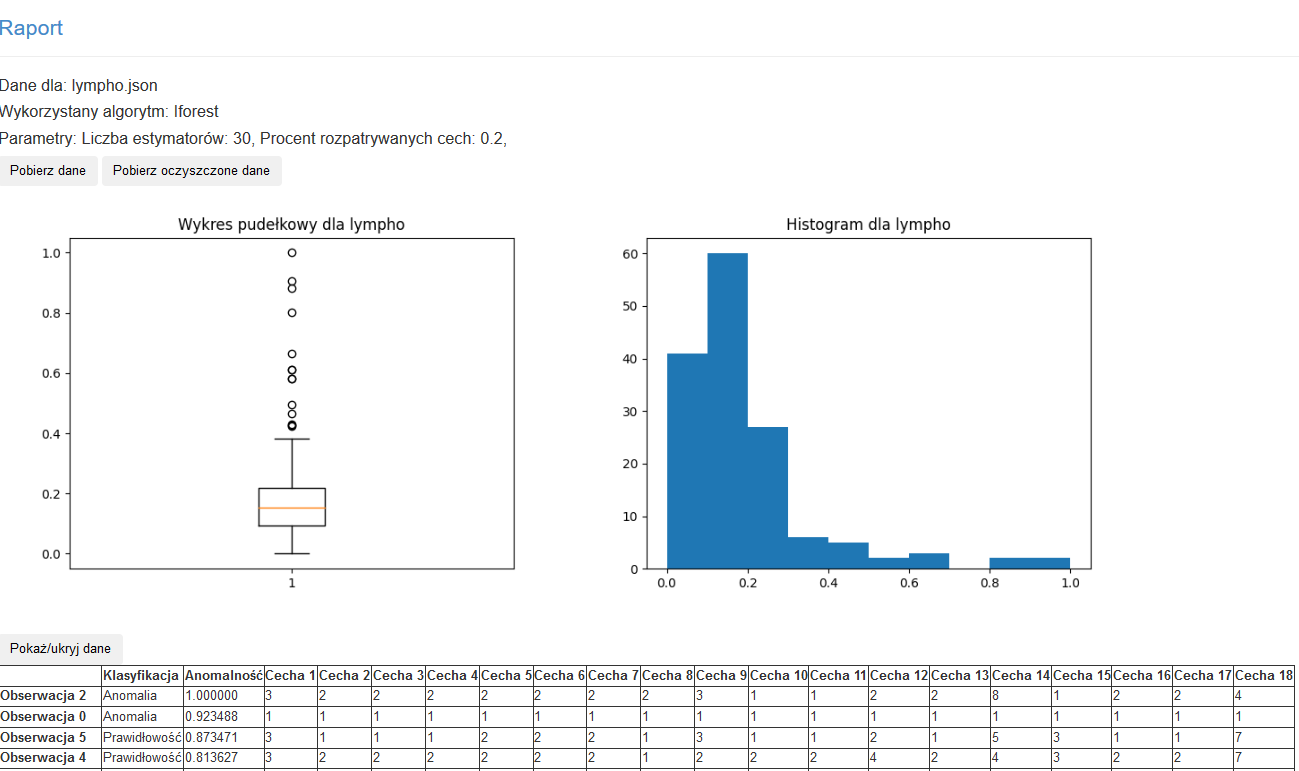
\includegraphics[width = \textwidth]{chapters/projekt/images/Screenshot_2021-01-29 Raport(3).png}
  \caption{Strona systemu po skończeniu zadania detekcji anomalii}
  \footnotesize{źródło: Opracowanie własne}
  \label{fig:label}
 \end{sidewaysfigure}

    % \chapter{Ewaluacja}

\begingroup
\leftskip4em
\rightskip\leftskip
\noindent
\textbf{Abstrakt} Rozdział przedstawia wyniki działania systemu oraz porównuje je z istniejącymi metodami wykrywania anomalii. Argumentuje wykorzystanie MinMaxScaler. Prezentuje możliwość rozwoju systemu.
\par
\endgroup

\section{Metryki do ewaluacji}
\section{Wyniki}
    % \chapter{Podsumowanie}
\label{chap:podsumowanie}
Tematyka wykrywania anomalii czy obserwacji odstających w polskiej literaturze naukowej jest niszowa. Detekcja anomalii z wykorzystaniem meta-uczenia jest innowacyjna.


% \begingroup
% \leftskip4em
% \rightskip\leftskip
% \noindent
% \textbf{Abstrakt} Żegnamy się 
% \par
% \endgroup


    
    \import{chapters/wstep/}{src.tex}
    \import{chapters/istniejace/}{src.tex}
    \import{chapters/MetaOD/}{src.tex}
    \import{chapters/projekt/}{src.tex}
    \import{chapters/analiza/}{src.tex}
    \import{chapters/ending/}{src.tex}
    
    % \appendixpage % Użyć tylko jeśli występuje więcej niż jeden dodatek!
    % \begin{appendix}
    %     \import{appendices/porownanie/}{src.tex}
    % \end{appendix}
    
    \addcontentsline{toc}{chapter}{\bibname}
    \bibliography{src/bibliography}

    \addcontentsline{toc}{chapter}{Spis rysunków}
    \listoffigures
    \addcontentsline{toc}{chapter}{Spis tablic}
    \listoftables
\end{document}

